% Options for packages loaded elsewhere
\PassOptionsToPackage{unicode}{hyperref}
\PassOptionsToPackage{hyphens}{url}
\PassOptionsToPackage{dvipsnames,svgnames,x11names}{xcolor}
%
\documentclass[
]{article}

\usepackage{amsmath,amssymb}
\usepackage{iftex}
\ifPDFTeX
  \usepackage[T1]{fontenc}
  \usepackage[utf8]{inputenc}
  \usepackage{textcomp} % provide euro and other symbols
\else % if luatex or xetex
  \usepackage{unicode-math}
  \defaultfontfeatures{Scale=MatchLowercase}
  \defaultfontfeatures[\rmfamily]{Ligatures=TeX,Scale=1}
\fi
\usepackage{lmodern}
\ifPDFTeX\else  
    % xetex/luatex font selection
\fi
% Use upquote if available, for straight quotes in verbatim environments
\IfFileExists{upquote.sty}{\usepackage{upquote}}{}
\IfFileExists{microtype.sty}{% use microtype if available
  \usepackage[]{microtype}
  \UseMicrotypeSet[protrusion]{basicmath} % disable protrusion for tt fonts
}{}
\makeatletter
\@ifundefined{KOMAClassName}{% if non-KOMA class
  \IfFileExists{parskip.sty}{%
    \usepackage{parskip}
  }{% else
    \setlength{\parindent}{0pt}
    \setlength{\parskip}{6pt plus 2pt minus 1pt}}
}{% if KOMA class
  \KOMAoptions{parskip=half}}
\makeatother
\usepackage{xcolor}
\setlength{\emergencystretch}{3em} % prevent overfull lines
\setcounter{secnumdepth}{-\maxdimen} % remove section numbering
% Make \paragraph and \subparagraph free-standing
\makeatletter
\ifx\paragraph\undefined\else
  \let\oldparagraph\paragraph
  \renewcommand{\paragraph}{
    \@ifstar
      \xxxParagraphStar
      \xxxParagraphNoStar
  }
  \newcommand{\xxxParagraphStar}[1]{\oldparagraph*{#1}\mbox{}}
  \newcommand{\xxxParagraphNoStar}[1]{\oldparagraph{#1}\mbox{}}
\fi
\ifx\subparagraph\undefined\else
  \let\oldsubparagraph\subparagraph
  \renewcommand{\subparagraph}{
    \@ifstar
      \xxxSubParagraphStar
      \xxxSubParagraphNoStar
  }
  \newcommand{\xxxSubParagraphStar}[1]{\oldsubparagraph*{#1}\mbox{}}
  \newcommand{\xxxSubParagraphNoStar}[1]{\oldsubparagraph{#1}\mbox{}}
\fi
\makeatother


\providecommand{\tightlist}{%
  \setlength{\itemsep}{0pt}\setlength{\parskip}{0pt}}\usepackage{longtable,booktabs,array}
\usepackage{calc} % for calculating minipage widths
% Correct order of tables after \paragraph or \subparagraph
\usepackage{etoolbox}
\makeatletter
\patchcmd\longtable{\par}{\if@noskipsec\mbox{}\fi\par}{}{}
\makeatother
% Allow footnotes in longtable head/foot
\IfFileExists{footnotehyper.sty}{\usepackage{footnotehyper}}{\usepackage{footnote}}
\makesavenoteenv{longtable}
\usepackage{graphicx}
\makeatletter
\def\maxwidth{\ifdim\Gin@nat@width>\linewidth\linewidth\else\Gin@nat@width\fi}
\def\maxheight{\ifdim\Gin@nat@height>\textheight\textheight\else\Gin@nat@height\fi}
\makeatother
% Scale images if necessary, so that they will not overflow the page
% margins by default, and it is still possible to overwrite the defaults
% using explicit options in \includegraphics[width, height, ...]{}
\setkeys{Gin}{width=\maxwidth,height=\maxheight,keepaspectratio}
% Set default figure placement to htbp
\makeatletter
\def\fps@figure{htbp}
\makeatother

\usepackage{float}
\usepackage{tabularray}
\usepackage[normalem]{ulem}
\usepackage{graphicx}
\UseTblrLibrary{booktabs}
\UseTblrLibrary{rotating}
\UseTblrLibrary{siunitx}
\NewTableCommand{\tinytableDefineColor}[3]{\definecolor{#1}{#2}{#3}}
\newcommand{\tinytableTabularrayUnderline}[1]{\underline{#1}}
\newcommand{\tinytableTabularrayStrikeout}[1]{\sout{#1}}
\makeatletter
\@ifpackageloaded{caption}{}{\usepackage{caption}}
\AtBeginDocument{%
\ifdefined\contentsname
  \renewcommand*\contentsname{Table of contents}
\else
  \newcommand\contentsname{Table of contents}
\fi
\ifdefined\listfigurename
  \renewcommand*\listfigurename{List of Figures}
\else
  \newcommand\listfigurename{List of Figures}
\fi
\ifdefined\listtablename
  \renewcommand*\listtablename{List of Tables}
\else
  \newcommand\listtablename{List of Tables}
\fi
\ifdefined\figurename
  \renewcommand*\figurename{Figure}
\else
  \newcommand\figurename{Figure}
\fi
\ifdefined\tablename
  \renewcommand*\tablename{Table}
\else
  \newcommand\tablename{Table}
\fi
}
\@ifpackageloaded{float}{}{\usepackage{float}}
\floatstyle{ruled}
\@ifundefined{c@chapter}{\newfloat{codelisting}{h}{lop}}{\newfloat{codelisting}{h}{lop}[chapter]}
\floatname{codelisting}{Listing}
\newcommand*\listoflistings{\listof{codelisting}{List of Listings}}
\makeatother
\makeatletter
\makeatother
\makeatletter
\@ifpackageloaded{caption}{}{\usepackage{caption}}
\@ifpackageloaded{subcaption}{}{\usepackage{subcaption}}
\makeatother

\ifLuaTeX
  \usepackage{selnolig}  % disable illegal ligatures
\fi
\usepackage{bookmark}

\IfFileExists{xurl.sty}{\usepackage{xurl}}{} % add URL line breaks if available
\urlstyle{same} % disable monospaced font for URLs
\hypersetup{
  pdftitle={HW3},
  pdfauthor={Miracle Ephraim},
  colorlinks=true,
  linkcolor={blue},
  filecolor={Maroon},
  citecolor={Blue},
  urlcolor={Blue},
  pdfcreator={LaTeX via pandoc}}


\title{HW3}
\author{Miracle Ephraim}
\date{}

\begin{document}
\maketitle


\section{Question 1}\label{question-1}

Present a bar graph showing the proportion of states with a change in
their cigarette tax in each year from 1970 to 1985.

\begin{verbatim}
Warning: Removed 1 row containing missing values or values outside the scale range
(`geom_col()`).
\end{verbatim}

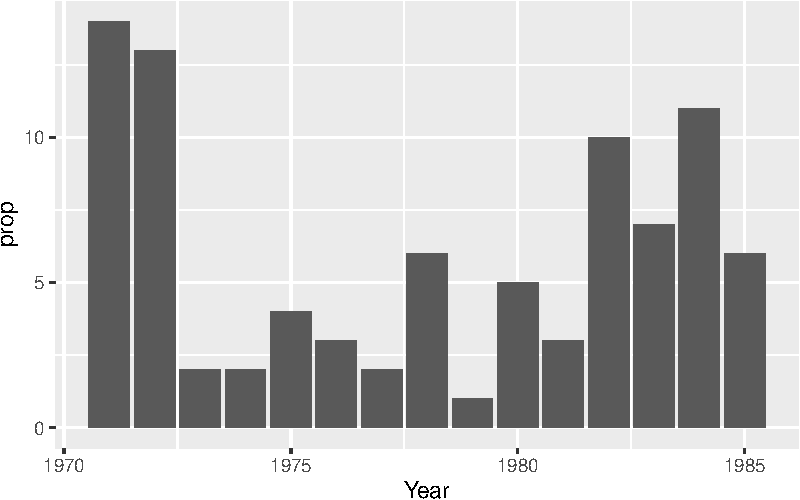
\includegraphics{ephraim-m-hwk3-3_files/figure-pdf/unnamed-chunk-1-1.pdf}

\section{Question 2}\label{question-2}

Plot on a single graph the average tax (in 2012 dollars) on cigarettes
and the average price of a pack of cigarettes from 1970 to 2018.

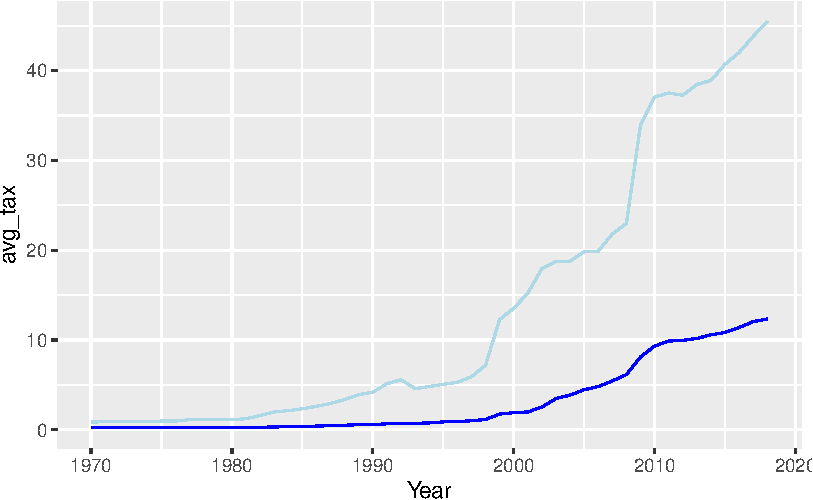
\includegraphics{ephraim-m-hwk3-3_files/figure-pdf/unnamed-chunk-2-1.pdf}

\section{Question 3}\label{question-3}

Identify the 5 states with the highest increases in cigarette prices (in
dollars) over the time period. Plot the average number of packs sold per
capita for those states from 1970 to 2018.

\begin{verbatim}
Warning: Returning more (or less) than 1 row per `summarise()` group was deprecated in
dplyr 1.1.0.
i Please use `reframe()` instead.
i When switching from `summarise()` to `reframe()`, remember that `reframe()`
  always returns an ungrouped data frame and adjust accordingly.
\end{verbatim}

\begin{verbatim}
`summarise()` has grouped output by 'state'. You can override using the
`.groups` argument.
\end{verbatim}

\begin{verbatim}
# A tibble: 5 x 2
# Groups:   state [5]
  state                 diff
  <chr>                <dbl>
1 District of Columbia  7.10
2 New York              7.01
3 Rhode Island          6.41
4 Hawaii                6.36
5 Massachusetts         6.36
\end{verbatim}

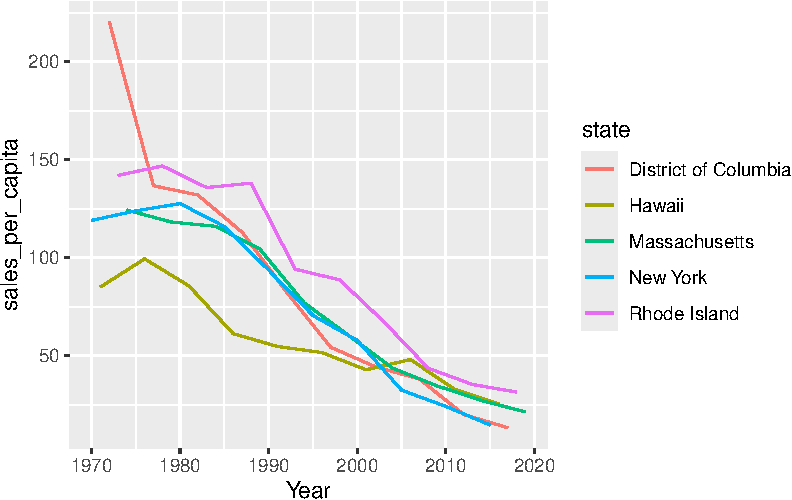
\includegraphics{ephraim-m-hwk3-3_files/figure-pdf/unnamed-chunk-3-1.pdf}

\section{Question 4}\label{question-4}

Identify the 5 states with the lowest increases in cigarette prices over
the time period. Plot the average number of packs sold per capita for
those states from 1970 to 2018.

\begin{verbatim}
Warning: Returning more (or less) than 1 row per `summarise()` group was deprecated in
dplyr 1.1.0.
i Please use `reframe()` instead.
i When switching from `summarise()` to `reframe()`, remember that `reframe()`
  always returns an ungrouped data frame and adjust accordingly.
\end{verbatim}

\begin{verbatim}
`summarise()` has grouped output by 'state'. You can override using the
`.groups` argument.
\end{verbatim}

\begin{verbatim}
# A tibble: 5 x 2
# Groups:   state [5]
  state           diff
  <chr>          <dbl>
1 Missouri        4.59
2 North Dakota    4.85
3 Tennessee       4.86
4 Georgia         4.87
5 North Carolina  4.88
\end{verbatim}

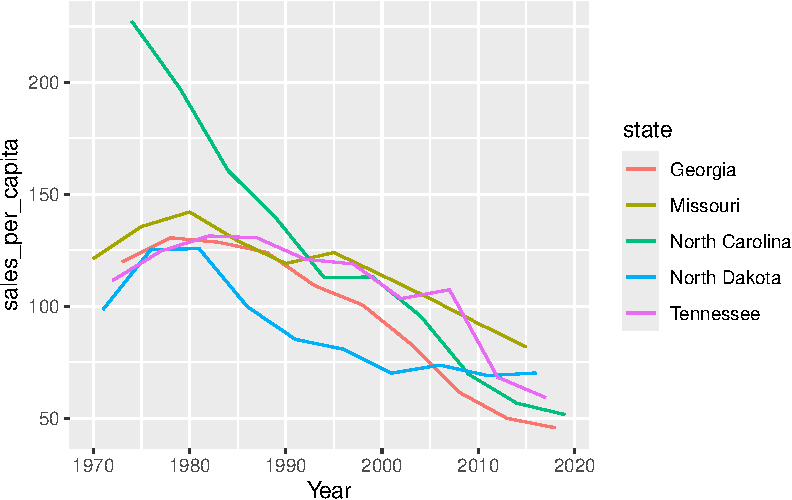
\includegraphics{ephraim-m-hwk3-3_files/figure-pdf/unnamed-chunk-4-1.pdf}

\section{Question 5}\label{question-5}

Compare the trends in sales from the 5 states with the highest price
increases to those with the lowest price increases.

In states with higher prices, average sales decrease at a much faster
rate compared to states where prices are lower.All states with high
prices see sales per capita drop below 50 by the early 2000s, while
states with lower reach that point by the end of follow-up (2018). These
findings demonstrate the significant effect price has on cigarette
sales, and are a good means of dissauding their use amongst the general
population.

\section{Question 6 - 9}\label{question-6---9}

\textbf{OLS + IV Estimates}

\begin{table}
\centering
\begin{talltblr}[         %% tabularray outer open
caption={Table 1: Elasticity Estimates from OLS and IV},
]                     %% tabularray outer close
{                     %% tabularray inner open
colspec={Q[]Q[]Q[]Q[]Q[]},
column{2,3,4,5}={}{halign=c,},
column{1}={}{halign=l,},
hline{6}={1,2,3,4,5}{solid, black, 0.05em},
}                     %% tabularray inner close
\toprule
& OLS (1970-1990) & IV (1970-1990) & OLS (1991-2015) & IV (1991-2015) \\ \midrule %% TinyTableHeader
log_cpi & -0.809 &  & -0.997 &  \\
& (0.038) &  & (0.025) &  \\
pricehat &  & -0.796 &  & -1.150 \\
&  & (0.081) &  & (0.026) \\
N & 1071 & 1071 & 1275 & 1275 \\
R² & 0.29 & 0.08 & 0.56 & 0.61 \\
\bottomrule
\end{talltblr}
\end{table}

OLS (1970 to 1990) On average, quantity demanded decreases by .02\% for
every 1\% increase in price.

IV (1970 to 1990) With a coefficient of -0.79, we can say price of
cigarettes is inelastic, with a 1\% increase in price leading to only
-0.79 change in quantity demanded. These are quite different from the
OLS estimates of elasticity, likely due to the endogeneity present in
the OLS model.

OLS (1990 to 2015) As price increases by 1\%, quantity demanded
decreases by .01\%.

IV (1990 to 2015)

With a coefficient of -1.15, we can say price of cigarettes is
inelastic, with a 1\% increase in price leading to a -1.15\% change in
quantity demanded. These are different from the OLS estimates of
elasticity as well, but not as stark of a contrast from the OLS
estimates.

\textbf{Reduced Form}

\begin{table}
\centering
\begin{talltblr}[         %% tabularray outer open
caption={Table 2: Reduced Form Estimates},
]                     %% tabularray outer close
{                     %% tabularray inner open
colspec={Q[]Q[]Q[]},
column{2,3}={}{halign=c,},
column{1}={}{halign=l,},
hline{4}={1,2,3}{solid, black, 0.05em},
}                     %% tabularray inner close
\toprule
& Reduced Form (1970-1990) & Reduced Form (1991-2015) \\ \midrule %% TinyTableHeader
log_total_tax & -0.207 & -0.591 \\
& (0.021) & (0.013) \\
N & 1071 & 1275 \\
R² & 0.08 & 0.61 \\
\bottomrule
\end{talltblr}
\end{table}

\begin{table}
\centering
\begin{talltblr}[         %% tabularray outer open
caption={Table 2: Reduced Form Estimates},
]                     %% tabularray outer close
{                     %% tabularray inner open
colspec={Q[]Q[]Q[]},
column{2,3}={}{halign=c,},
column{1}={}{halign=l,},
hline{4}={1,2,3}{solid, black, 0.05em},
}                     %% tabularray inner close
\toprule
& Reduced Form (1970-1990) & Reduced Form (1991-2015) \\ \midrule %% TinyTableHeader
log_total_tax & -0.207 & -0.591 \\
& (0.021) & (0.013) \\
N & 1071 & 1275 \\
R² & 0.08 & 0.61 \\
\bottomrule
\end{talltblr}
\end{table}

\section{Question 10}\label{question-10}

Compare your elasticity estimates from 1970-1990 versus those from
1991-2015. Are they different? If so, why?

The estimates from each 20-year period are different from eachother,
likely due to changes in attitudes around smoking and the increasing
taxes placed on the product.

\textbf{Github Repo:} {[}https://github.com/miracleephraim/hw3.git{]}
(https://github.com/miracleephraim/hw3.git)




\end{document}
